% =====================================================================
% IEEE Conference Paper — Cassava Leaf Disease Classification
% Authors: Ali Baki Türköz, Emre Öztürk (Özyeğin University, MSc CS)
% Course: CS523 — Computer Vision
%
% Compile with pdfLaTeX on Overleaf:
%   - Set TeX Live version to latest
%   - Main document type: pdfLaTeX
%   - Bibliography is BibTeX (filecontents block at top)
% =====================================================================

\documentclass[conference]{IEEEtran}
\IEEEoverridecommandlockouts

% ---------- Packages ----------
\usepackage{cite}
\usepackage{amsmath,amssymb,amsfonts}
\usepackage{algorithmic}
\usepackage{graphicx}
\usepackage{textcomp}
\usepackage{xcolor}
\usepackage{booktabs}
\usepackage{multirow}
\usepackage{array}
\usepackage{url}
\usepackage{hyperref}
\hypersetup{
    colorlinks=true,
    linkcolor=black,
    citecolor=black,
    urlcolor=blue,
}

\def\BibTeX{{\rm B\kern-.05em{\sc i\kern-.025em b}\kern-.08em
    T\kern-.1667em\lower.7ex\hbox{E}\kern-.125emX}}

% =====================================================================
% Inline bibliography (so Overleaf needs only this single .tex file)
% =====================================================================
\begin{filecontents*}{references.bib}
@inproceedings{he2016resnet,
  author    = {He, Kaiming and Zhang, Xiangyu and Ren, Shaoqing and Sun, Jian},
  title     = {Deep Residual Learning for Image Recognition},
  booktitle = {Proceedings of the IEEE Conference on Computer Vision and Pattern Recognition (CVPR)},
  year      = {2016},
  pages     = {770--778}
}
@inproceedings{tan2019efficientnet,
  author    = {Tan, Mingxing and Le, Quoc V.},
  title     = {{EfficientNet}: Rethinking Model Scaling for Convolutional Neural Networks},
  booktitle = {Proceedings of the 36th International Conference on Machine Learning (ICML)},
  year      = {2019},
  pages     = {6105--6114}
}
@inproceedings{dosovitskiy2021vit,
  author    = {Dosovitskiy, Alexey and Beyer, Lucas and Kolesnikov, Alexander and Weissenborn, Dirk and Zhai, Xiaohua and Unterthiner, Thomas and Dehghani, Mostafa and Minderer, Matthias and Heigold, Georg and Gelly, Sylvain and Uszkoreit, Jakob and Houlsby, Neil},
  title     = {An Image is Worth 16x16 Words: Transformers for Image Recognition at Scale},
  booktitle = {International Conference on Learning Representations (ICLR)},
  year      = {2021}
}
@inproceedings{deng2009imagenet,
  author    = {Deng, Jia and Dong, Wei and Socher, Richard and Li, Li-Jia and Li, Kai and Fei-Fei, Li},
  title     = {{ImageNet}: A Large-Scale Hierarchical Image Database},
  booktitle = {IEEE Conference on Computer Vision and Pattern Recognition (CVPR)},
  year      = {2009},
  pages     = {248--255}
}
@article{mohanty2016plantdisease,
  author    = {Mohanty, Sharada P. and Hughes, David P. and Salath\'{e}, Marcel},
  title     = {Using Deep Learning for Image-Based Plant Disease Detection},
  journal   = {Frontiers in Plant Science},
  year      = {2016},
  volume    = {7},
  pages     = {1419}
}
@article{ferentinos2018,
  author    = {Ferentinos, Konstantinos P.},
  title     = {Deep Learning Models for Plant Disease Detection and Diagnosis},
  journal   = {Computers and Electronics in Agriculture},
  year      = {2018},
  volume    = {145},
  pages     = {311--318}
}
@article{barbedo2018,
  author    = {Barbedo, Jayme G. A.},
  title     = {Factors Influencing the Use of Deep Learning for Plant Disease Recognition},
  journal   = {Biosystems Engineering},
  year      = {2018},
  volume    = {172},
  pages     = {84--91}
}
@article{mwebaze2020cassava,
  author    = {Mwebaze, Ernest and Gebru, Timnit and Frome, Andrea and Nsumba, Solomon and Tusubira, Jeremy},
  title     = {{iCassava 2019} Fine-Grained Visual Categorization Challenge},
  journal   = {arXiv preprint arXiv:1908.02900},
  year      = {2019}
}
@inproceedings{akiba2019optuna,
  author    = {Akiba, Takuya and Sano, Shotaro and Yanase, Toshihiko and Ohta, Takeru and Koyama, Masanori},
  title     = {{Optuna}: A Next-Generation Hyperparameter Optimization Framework},
  booktitle = {Proceedings of the 25th ACM SIGKDD International Conference on Knowledge Discovery and Data Mining (KDD)},
  year      = {2019},
  pages     = {2623--2631}
}
@inproceedings{lin2017focal,
  author    = {Lin, Tsung-Yi and Goyal, Priya and Girshick, Ross and He, Kaiming and Doll\'{a}r, Piotr},
  title     = {Focal Loss for Dense Object Detection},
  booktitle = {Proceedings of the IEEE International Conference on Computer Vision (ICCV)},
  year      = {2017},
  pages     = {2980--2988}
}
@inproceedings{szegedy2016label,
  author    = {Szegedy, Christian and Vanhoucke, Vincent and Ioffe, Sergey and Shlens, Jon and Wojna, Zbigniew},
  title     = {Rethinking the {Inception} Architecture for Computer Vision},
  booktitle = {Proceedings of the IEEE Conference on Computer Vision and Pattern Recognition (CVPR)},
  year      = {2016},
  pages     = {2818--2826}
}
@inproceedings{loshchilov2019adamw,
  author    = {Loshchilov, Ilya and Hutter, Frank},
  title     = {Decoupled Weight Decay Regularization},
  booktitle = {International Conference on Learning Representations (ICLR)},
  year      = {2019}
}
@inproceedings{loshchilov2017sgdr,
  author    = {Loshchilov, Ilya and Hutter, Frank},
  title     = {{SGDR}: Stochastic Gradient Descent with Warm Restarts},
  booktitle = {International Conference on Learning Representations (ICLR)},
  year      = {2017}
}
@inproceedings{micikevicius2018mixed,
  author    = {Micikevicius, Paulius and Narang, Sharan and Alben, Jonah and Diamos, Gregory and Elsen, Erich and Garcia, David and Ginsburg, Boris and Houston, Michael and Kuchaiev, Oleksii and Venkatesh, Ganesh and Wu, Hao},
  title     = {Mixed Precision Training},
  booktitle = {International Conference on Learning Representations (ICLR)},
  year      = {2018}
}
@article{cortes1995svm,
  author    = {Cortes, Corinna and Vapnik, Vladimir},
  title     = {Support-Vector Networks},
  journal   = {Machine Learning},
  year      = {1995},
  volume    = {20},
  number    = {3},
  pages     = {273--297}
}
@article{breiman2001randomforests,
  author    = {Breiman, Leo},
  title     = {Random Forests},
  journal   = {Machine Learning},
  year      = {2001},
  volume    = {45},
  number    = {1},
  pages     = {5--32}
}
@inproceedings{chen2016xgboost,
  author    = {Chen, Tianqi and Guestrin, Carlos},
  title     = {{XGBoost}: A Scalable Tree Boosting System},
  booktitle = {Proceedings of the 22nd ACM SIGKDD International Conference on Knowledge Discovery and Data Mining (KDD)},
  year      = {2016},
  pages     = {785--794}
}
@inproceedings{zhong2020randomerasing,
  author    = {Zhong, Zhun and Zheng, Liang and Kang, Guoliang and Li, Shaozi and Yang, Yi},
  title     = {Random Erasing Data Augmentation},
  booktitle = {Proceedings of the AAAI Conference on Artificial Intelligence},
  year      = {2020}
}
\end{filecontents*}

% =====================================================================
% Title and Authors
% =====================================================================
\begin{document}

\title{Cassava Leaf Disease Classification}

\author{
\IEEEauthorblockN{Ali Baki T\"{u}rk\"{o}z}
\IEEEauthorblockA{Department of Computer Science \\
M.Sc.\ Program \\
\"{O}zye\u{g}in University \\
Istanbul, T\"{u}rkiye \\
baki.turkoz@ozu.edu.tr}
\and
\IEEEauthorblockN{Emre \"{O}zt\"{u}rk}
\IEEEauthorblockA{Department of Computer Science \\
M.Sc.\ Program \\
\"{O}zye\u{g}in University \\
Istanbul, T\"{u}rkiye \\
emre.ozturk.46760@ozu.edu.tr}
}

\maketitle

% =====================================================================
% Abstract
% =====================================================================
\begin{abstract}
Plant disease detection is a critical task in agriculture, directly affecting crop yield and global food security. Cassava, a staple crop in tropical regions, is particularly vulnerable to several diseases that share visually similar leaf-level symptoms, making manual diagnosis costly and error-prone. In this work, we present a systematic comparative analysis of three families of image-classification approaches for the Cassava Leaf Disease Classification (CLDC) benchmark, which contains approximately 21{,}397 field-acquired images distributed across five strongly imbalanced classes. Specifically, we compare (i)~classical machine-learning baselines (Support Vector Machine, Random Forest, XGBoost) operating on grayscale Principal-Component-Analysis features, (ii)~a convolutional baseline (ResNet-50) and a stronger convolutional architecture (EfficientNet-B4), and (iii)~a transformer-based architecture (Vision Transformer, ViT-B/16). All deep models are fine-tuned from ImageNet-pretrained weights under a fully reproducible 3-fold stratified cross-validation protocol, with class-imbalance handling, mixed-precision training, and early stopping. A categorical Optuna-driven hyperparameter search (Tree-structured Parzen Estimator with median pruning) is conducted over learning rate, weight decay, batch size, loss function (cross-entropy, label-smoothed cross-entropy, focal loss), optimizer (AdamW, Adam, SGD with Nesterov momentum), and learning-rate scheduler. Two complementary ablation studies are performed: (a)~an extensive data-augmentation sweep comprising 22 different augmentation policies grouped into baseline, single-component, competition-derived, and combined categories, and (b)~an analysis of the impact of class-balanced versus unbalanced loss weighting. Performance is reported using accuracy, macro/weighted precision, recall, F1-score, and per-class metrics, together with confusion matrices and learning curves. This proposal describes the full methodological pipeline and the experimental design; experimental findings will be reported in the final paper.
\end{abstract}

\begin{IEEEkeywords}
plant disease classification, cassava leaf disease, convolutional neural networks, vision transformer, transfer learning, Optuna, hyperparameter optimization, data augmentation, class imbalance, ablation study.
\end{IEEEkeywords}

% =====================================================================
% Introduction
% =====================================================================
\section{Introduction}
\label{sec:intro}

Agriculture remains a key pillar of global food security, and crop diseases continue to account for substantial yield losses worldwide. Among staple crops cultivated in tropical regions, cassava (\emph{Manihot esculenta}) is particularly important: it provides a major source of carbohydrates for millions of producers in sub-Saharan Africa. However, cassava is highly susceptible to a number of viral, bacterial, and arthropod-mediated diseases, including Cassava Bacterial Blight (CBB), Cassava Brown Streak Disease (CBSD), Cassava Green Mottle (CGM), and Cassava Mosaic Disease (CMD)~\cite{mwebaze2020cassava}. Early and accurate identification of these diseases is essential for limiting losses, yet expert-driven manual inspection is expensive, slow, and difficult to scale.

Computer-vision-based automated disease detection offers a practical alternative. Deep convolutional neural networks (CNNs) have produced strong results in plant-disease classification under controlled laboratory conditions~\cite{mohanty2016plantdisease,ferentinos2018}, but generalization to images taken with mobile phones in farmers' fields---under varying illumination, complex backgrounds, motion blur, and label noise---remains an open challenge~\cite{barbedo2018}. The Cassava Leaf Disease Classification (CLDC) dataset~\cite{mwebaze2020cassava}, released through a Kaggle competition, captures exactly these real-world difficulties. It contains roughly $21{,}397$ images across five classes and exhibits severe class imbalance, with the CMD class accounting for more than $61\%$ of the data while the rarest class (CBB) accounts for only about $5\%$.

Recent advances in computer vision have introduced two complementary directions worth investigating on this benchmark. On the convolutional side, EfficientNet~\cite{tan2019efficientnet} provides a principled compound-scaling rule that obtains higher accuracy than ResNet-style backbones~\cite{he2016resnet} at comparable parameter budgets. On the architectural side, the Vision Transformer (ViT)~\cite{dosovitskiy2021vit} demonstrates that pure self-attention models, when pretrained on large-scale data, can match or exceed convolutional models on image classification. Whether these gains transfer to a noisy, imbalanced, in-the-wild agricultural domain such as cassava is a question that motivates this study.

In parallel, training-protocol decisions---such as the choice of optimizer, learning-rate schedule, loss function, and data-augmentation strategy---are known to have a comparable or even larger impact on final performance than the choice of backbone~\cite{loshchilov2019adamw,loshchilov2017sgdr,lin2017focal}. In settings with strong class imbalance and limited annotated samples, principled hyperparameter search and careful augmentation design are therefore not optional. This proposal addresses these considerations directly through an Optuna-based~\cite{akiba2019optuna} categorical search over hyperparameters and an explicit augmentation ablation.

The main contributions of this work, as planned, are the following:
\begin{itemize}
  \item We provide a controlled, fully reproducible comparison of three deep-learning architectures (ResNet-50, EfficientNet-B4, ViT-B/16) on CLDC under a unified 3-fold stratified cross-validation protocol, with class-weight handling, mixed-precision training, early stopping, and seed determinism.
  \item We include classical machine-learning baselines (SVM, Random Forest, XGBoost) operating on grayscale flattened pixels with Principal-Component-Analysis (PCA) dimensionality reduction, to quantify the gap between handcrafted-feature classifiers and deep models on this task.
  \item We perform a categorical hyperparameter search using the Optuna framework with a Tree-structured Parzen Estimator (TPE) sampler and a median pruner, jointly searching over learning rate, weight decay, batch size, optimizer, loss function (including focal and label-smoothed variants), and learning-rate scheduler.
  \item We perform two complementary ablation studies that target the principal sources of variation specific to this dataset: (i)~a 22-mode data-augmentation sweep covering baseline, single-component, competition-derived, and combined policies, and (ii)~a class-weighting ablation that contrasts class-balanced versus unweighted loss training.
\end{itemize}

The remainder of this proposal is organized as follows. Section~\ref{sec:related} reviews related work in plant-disease classification, transfer learning, and hyperparameter optimization. Section~\ref{sec:method} describes the proposed methodology in detail, including the dataset, models, training protocol, hyperparameter search procedure, and ablation design. Experimental results, comparative analysis, and discussion will be presented in the final paper.

% =====================================================================
% Related Work
% =====================================================================
\section{Related Work}
\label{sec:related}

\subsection{Deep Learning for Plant Disease Classification}
The application of deep learning to plant-disease recognition was popularized by Mohanty \emph{et al.}~\cite{mohanty2016plantdisease}, who trained AlexNet- and GoogLeNet-style networks on the PlantVillage dataset and reported test accuracies above $99\%$ on lab-controlled images. Ferentinos~\cite{ferentinos2018} extended this analysis to multiple CNN backbones and a larger collection of plant species, confirming that pretrained CNNs strongly outperform classical pipelines on clean, controlled-environment images. However, Barbedo~\cite{barbedo2018} explicitly identified the limitations of these studies in real-world conditions, arguing that performance degrades substantially when the test distribution includes complex backgrounds, mixed illumination, and label noise. The CLDC benchmark~\cite{mwebaze2020cassava}, captured by farmers using mobile devices, exhibits exactly the failure modes Barbedo emphasized, making it a more demanding test bed than PlantVillage and a natural target for the architectures evaluated in this work.

\subsection{Convolutional and Transformer Backbones}
Residual learning~\cite{he2016resnet} remains a standard reference architecture for image classification: ResNet-50 in particular is widely adopted as a strong, well-understood baseline in transfer-learning studies. EfficientNet~\cite{tan2019efficientnet} introduces a compound-scaling rule that jointly increases network depth, width, and resolution, achieving improved accuracy--efficiency trade-offs across the EfficientNet-B0 to EfficientNet-B7 family. The Vision Transformer (ViT)~\cite{dosovitskiy2021vit} discards convolutional inductive biases altogether and instead processes images as sequences of $16{\times}16$ patches with multi-head self-attention. When pretrained on large-scale corpora (e.g., ImageNet-21k or JFT-300M~\cite{deng2009imagenet}), ViT matches or exceeds the accuracy of state-of-the-art CNNs on multiple benchmarks. The relative performance of these three architectures on a noisy, imbalanced agricultural dataset is one of the questions this work seeks to answer empirically.

\subsection{Class Imbalance Handling}
Class imbalance is a recurring challenge in real-world classification, and CLDC is a strongly imbalanced benchmark. Two main families of mitigations are relevant here. The first is loss reweighting: assigning class weights inversely proportional to class frequency in the standard cross-entropy objective. The second is loss reshaping: the focal loss of Lin \emph{et al.}~\cite{lin2017focal} introduces a modulating factor $(1-p_t)^\gamma$ that down-weights well-classified examples and focuses gradient updates on hard or minority examples. A related but distinct regularizer, label smoothing~\cite{szegedy2016label}, replaces hard one-hot targets with smoothed distributions and is known to improve calibration and generalization on noisy-label datasets. This work compares all three loss formulations.

\subsection{Hyperparameter Optimization}
Modern deep-learning pipelines have many interacting hyperparameters, and grid or manual tuning is rarely competitive. Optuna~\cite{akiba2019optuna} provides a define-by-run framework that combines Bayesian search via the Tree-structured Parzen Estimator with median-based pruning of unpromising trials, yielding substantial speedups over uniform random search. We adopt this framework to jointly search over optimization-related hyperparameters in a categorical search space. On the optimizer side, AdamW~\cite{loshchilov2019adamw} decouples weight decay from the gradient update of Adam and is now the de-facto default for transformer fine-tuning. On the scheduler side, ReduceLROnPlateau, cosine annealing, and cosine annealing with warm restarts (SGDR)~\cite{loshchilov2017sgdr} are all standard choices for image classification and are included in our search.

\subsection{Data Augmentation and Mixed-Precision Training}
Data augmentation is a primary tool for improving generalization on small or noisy datasets. Beyond standard geometric transforms (flips, rotation, scale jitter) and photometric transforms (color jitter, brightness/contrast adjustment), Random Erasing~\cite{zhong2020randomerasing} simulates partial occlusion by replacing rectangular regions of the input image with noise or a constant value; this has been reported to improve robustness on fine-grained agricultural images, including in top-performing CLDC competition solutions. Mixed-precision training~\cite{micikevicius2018mixed} uses half-precision floating-point arithmetic for the forward and backward passes while maintaining a master copy of the weights in full precision, reducing memory consumption and roughly doubling training throughput on modern GPUs. We adopt mixed precision throughout to make the Optuna-driven sweep computationally tractable.

\subsection{Classical Baselines}
For completeness, we also evaluate classical machine-learning baselines based on raw-pixel features. Support Vector Machines~\cite{cortes1995svm} with RBF kernels, Random Forests~\cite{breiman2001randomforests}, and gradient-boosted decision trees as implemented in XGBoost~\cite{chen2016xgboost} are well-established, strong non-deep classifiers and are widely used as reference baselines when assessing the value added by deep learning on a given problem.

% =====================================================================
% Method
% =====================================================================
\section{Methodology}
\label{sec:method}

\subsection{Dataset}
\label{ssec:data}
We use the Cassava Leaf Disease Classification (CLDC) dataset~\cite{mwebaze2020cassava} released through a Kaggle competition. The dataset comprises approximately $21{,}397$ field-acquired RGB images of cassava leaves, captured by farmers using mobile phones under uncontrolled illumination, varying backgrounds, partial occlusion, and varying image quality. Each image is labeled with one of five mutually exclusive classes. Fig.~\ref{fig:class_dist} reports the per-class image counts and proportions in the training metadata used in this work, and Fig.~\ref{fig:samples} shows one representative image from each class.

\begin{figure}[t]
\centering
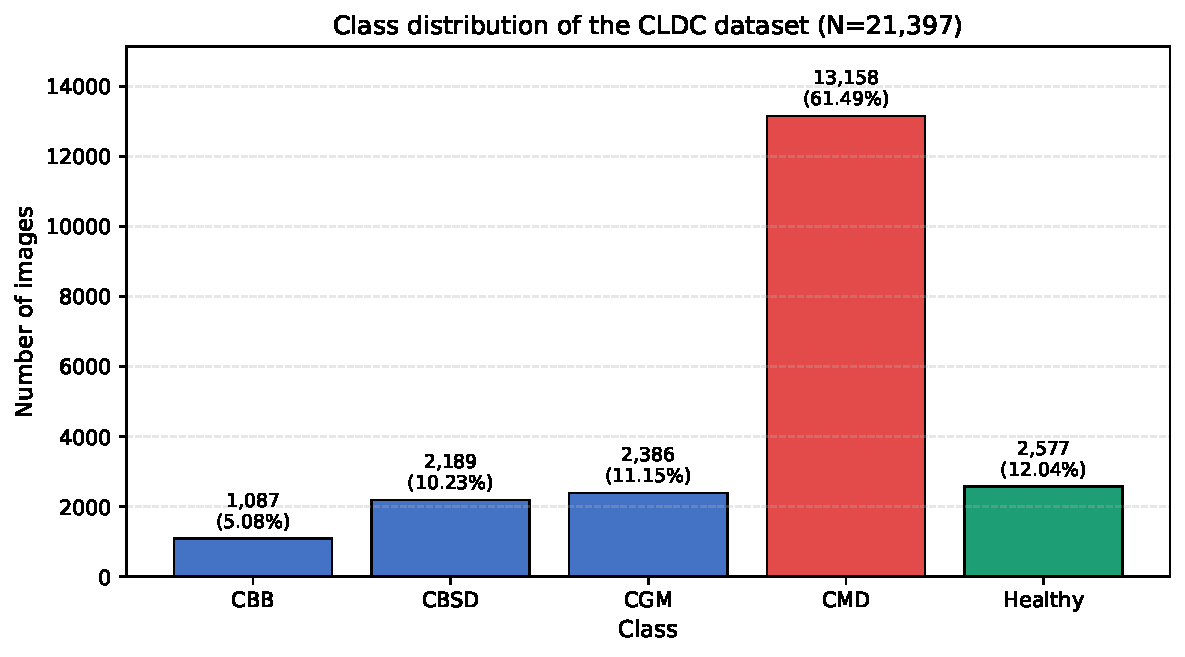
\includegraphics[width=\linewidth]{fig/fig_class_distribution.pdf}
\caption{Class distribution of the CLDC dataset used in this work. The Cassava Mosaic Disease (CMD) class accounts for $61.49\%$ of the data, while the rarest class (CBB) accounts for only $5.08\%$; the ratio between the largest and smallest classes is approximately $12{:}1$.}
\label{fig:class_dist}
\end{figure}

\begin{figure}[t]
\centering
\setlength{\tabcolsep}{2pt}
\begin{tabular}{ccccc}
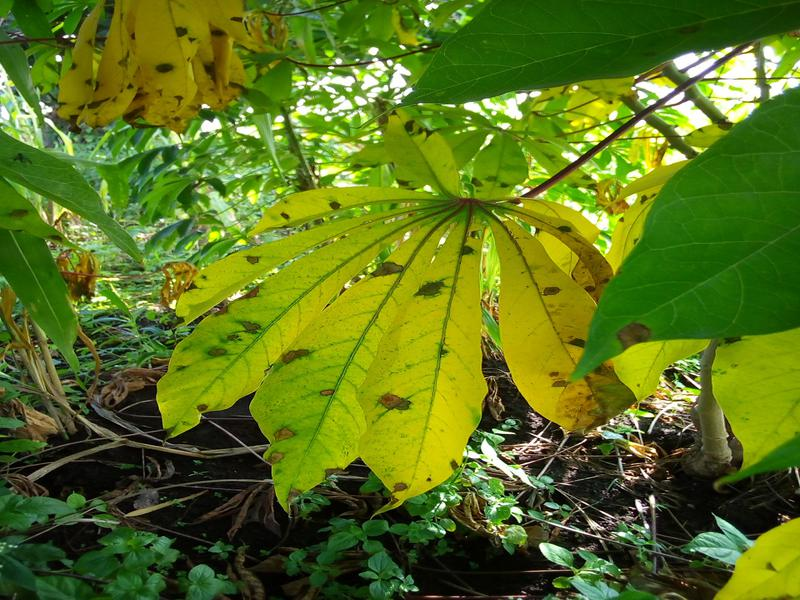
\includegraphics[width=0.165\linewidth]{fig/examples/label0_Cassava_Bacterial_Blight_CBB_2292154193.jpg} &
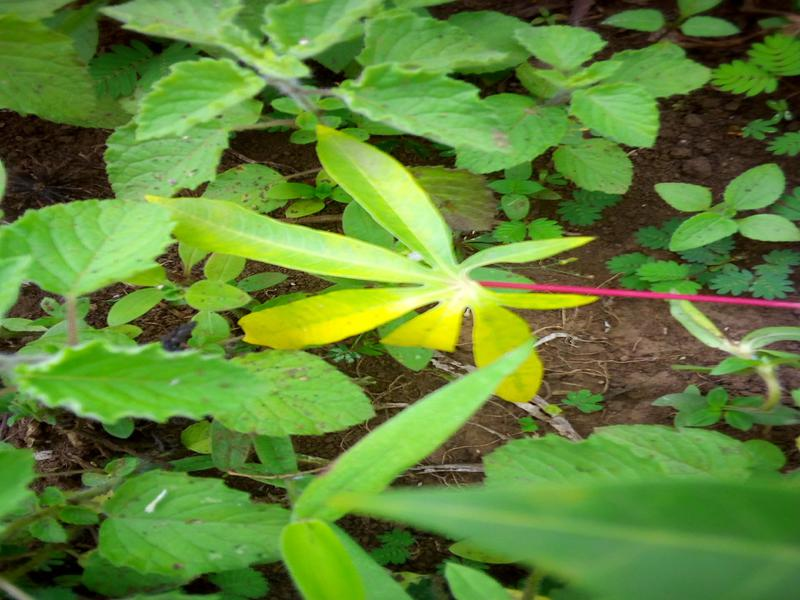
\includegraphics[width=0.165\linewidth]{fig/examples/label1_Cassava_Brown_Streak_Disease_CBSD_1053506407.jpg} &
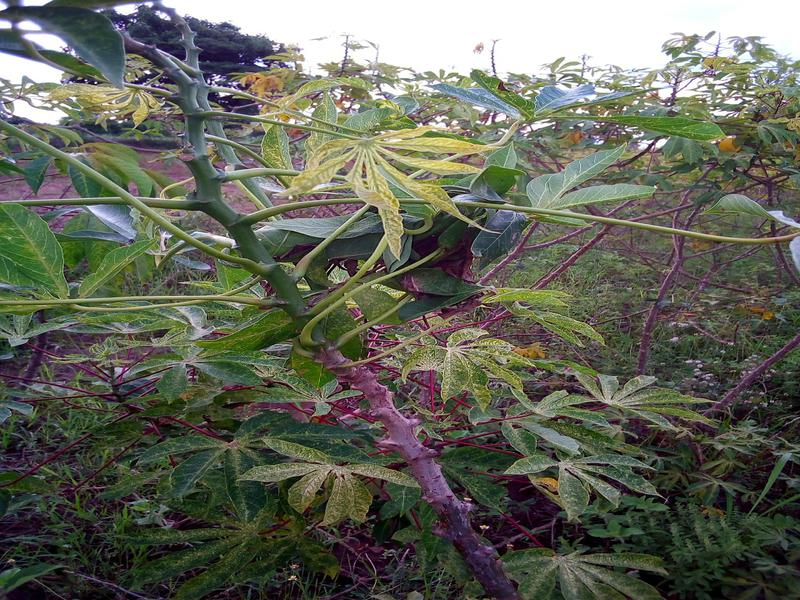
\includegraphics[width=0.165\linewidth]{fig/examples/label2_Cassava_Green_Mottle_CGM_532304081.jpg} &
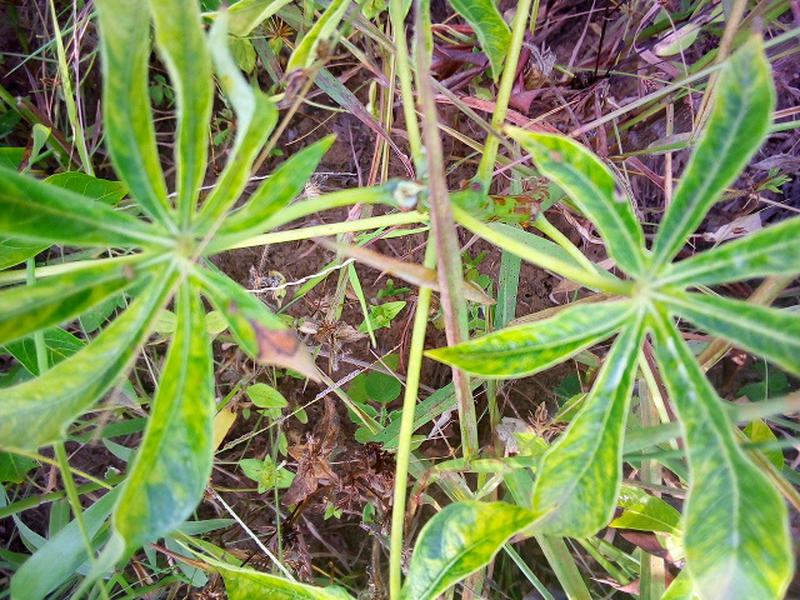
\includegraphics[width=0.165\linewidth]{fig/examples/label3_Cassava_Mosaic_Disease_CMD_575135832.jpg} &
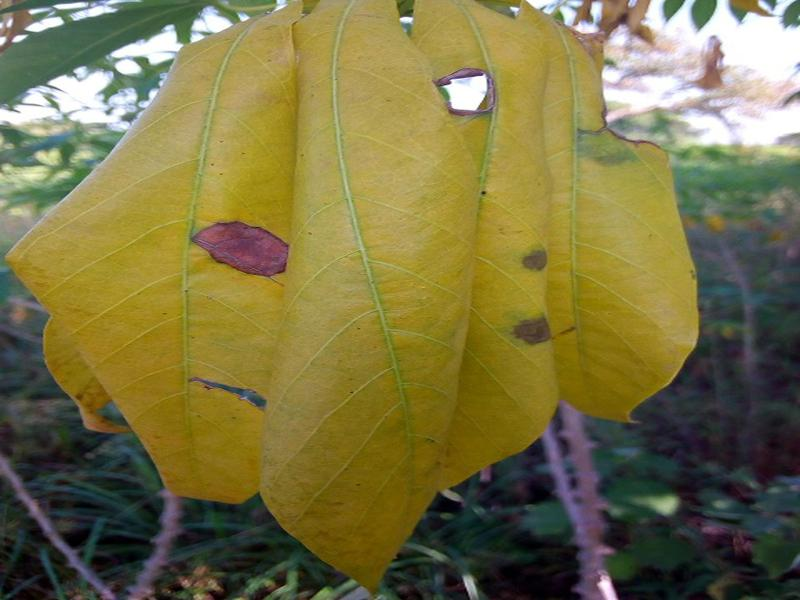
\includegraphics[width=0.165\linewidth]{fig/examples/label4_Healthy_1372417670.jpg} \\
\footnotesize CBB & \footnotesize CBSD & \footnotesize CGM & \footnotesize CMD & \footnotesize Healthy \\
\end{tabular}
\caption{Representative training images, one per class. The visual similarity between several disease classes, together with cluttered backgrounds and varying illumination, illustrates the difficulty of the CLDC benchmark.}
\label{fig:samples}
\end{figure}

The dataset is highly imbalanced: the CMD class alone accounts for $61.49\%$ of the training data, while the rarest class (CBB) accounts for only $5.08\%$. The ratio between the largest and smallest classes is approximately $12{:}1$. This imbalance, together with the in-the-wild acquisition conditions, motivates the class-weighting, focal-loss, and augmentation strategies described below.

\subsection{Evaluation Protocol}
\label{ssec:eval}
We use \emph{3-fold stratified cross-validation} as the sole evaluation protocol; no separate held-out test split is used. Stratification preserves the per-class proportions of Fig.~\ref{fig:class_dist} within each fold. For every experimental condition (every Optuna trial and every augmentation policy in the ablation), the full pipeline is repeated three times: training on two folds and evaluating on the held-out third. The reported metrics are the mean and standard deviation across the three folds. This corresponds to using out-of-fold validation predictions as a proxy for held-out test performance and is the same protocol referenced in the project proposal as the ``optional k-fold cross-validation'' alternative to a fixed split.

For each fold, we record accuracy, macro-averaged precision, recall, and F1-score, the corresponding weighted-averaged metrics, and per-class precision, recall, and F1. We also record the full $5{\times}5$ confusion matrix and the training/validation loss and accuracy curves. Macro-averaged F1 (\texttt{f1\_macro}) is the primary metric used both as the Optuna objective and as the headline comparison criterion, because it weighs all classes equally and is therefore appropriate for the strongly imbalanced CLDC class distribution. Accuracy, in contrast, is dominated by the majority CMD class and is reported as a secondary metric only.

\subsection{Models}
\label{ssec:models}

\paragraph{Classical baselines.}
For the classical pipeline, each image is converted to grayscale, resized to $64{\times}64$ pixels, scaled to $[0,1]$, and flattened to a $4{,}096$-dimensional feature vector. A single \texttt{StandardScaler} $\rightarrow$ \texttt{PCA(0.95 variance)} $\rightarrow$ classifier pipeline is then fit per fold. Three classifiers are evaluated: a Support Vector Machine~\cite{cortes1995svm} with RBF kernel and the \texttt{class\_weight=balanced} option; a Random Forest~\cite{breiman2001randomforests} with $300$ trees and \texttt{class\_weight=balanced}; and an XGBoost~\cite{chen2016xgboost} classifier with $300$ boosting rounds, depth-$6$ trees, learning rate $0.1$, and per-sample class-balancing weights computed from the training fold. These baselines deliberately use a small input resolution and a single global feature representation; they are intended as a lower-bound reference, not as competitive solutions.

\paragraph{Deep models.}
Three pretrained backbones are fine-tuned end-to-end. ResNet-50~\cite{he2016resnet} is loaded from \texttt{torchvision} with ImageNet-1k V2 weights; its final fully connected layer is replaced by a five-way classifier and the input resolution is set to $224{\times}224$. EfficientNet-B4~\cite{tan2019efficientnet} is loaded with ImageNet-1k weights; the final linear layer of its classifier head is replaced and the input resolution is also set to $224{\times}224$ to keep memory cost comparable. ViT-B/16~\cite{dosovitskiy2021vit} is loaded with ImageNet-1k weights and its classification head is replaced; following the architecture's design, the input resolution is set to $384{\times}384$. In all three cases, every parameter is set as trainable (no layer freezing); this corresponds to full fine-tuning.

\subsection{Training Protocol}
\label{ssec:training}

All deep models are trained with the same shared infrastructure, which differs only in the categorical hyperparameters chosen by Optuna. The base elements are the following.

\paragraph{Reproducibility.}
A single global seed is set for Python's \texttt{random} module, NumPy, PyTorch (CPU and CUDA), and \texttt{PYTHONHASHSEED}. Deterministic cuDNN kernels are enabled, the cuBLAS workspace is configured for determinism, and PyTorch's \texttt{use\_deterministic\_algorithms} flag is activated. DataLoader workers are seeded individually. These settings produce bit-level reproducible runs at the cost of modest throughput.

\paragraph{Mixed precision.}
Training and inference are run under PyTorch's \texttt{torch.amp.autocast} with \texttt{float16} computation and a master copy of weights in \texttt{float32}, as introduced by Micikevicius \emph{et al.}~\cite{micikevicius2018mixed}. A \texttt{GradScaler} is used to prevent gradient underflow.

\paragraph{Class-imbalance handling.}
For each training fold, per-class weights $w_c = N / (C \cdot n_c)$ are computed from the fold's label distribution, where $N$ is the number of training examples, $C=5$ is the number of classes, and $n_c$ is the count of class $c$. These weights are used either directly inside the loss (cross-entropy, label-smoothed cross-entropy, focal loss) or---in the unbalanced control condition---disabled. The \texttt{use\_class\_weights} flag is part of the ablation study described in Section~\ref{ssec:ablation}.

\paragraph{Loss functions.}
We compare three loss families:
\begin{itemize}
  \item \emph{Cross-entropy} with class weights (the baseline objective).
  \item \emph{Label-smoothed cross-entropy}~\cite{szegedy2016label} with smoothing parameter $\varepsilon \in \{0.05, 0.10, 0.20\}$.
  \item \emph{Focal loss}~\cite{lin2017focal} of the form
        $\mathrm{FL}(p_t) = -\alpha_t (1-p_t)^{\gamma} \log p_t$,
        with $\gamma \in \{1.0, 1.5, 2.0, 2.5\}$ and $\alpha_t$ taken from the class-balanced weights above.
\end{itemize}

\paragraph{Optimizers and schedulers.}
The search space includes AdamW~\cite{loshchilov2019adamw}, Adam, and SGD with Nesterov momentum, with momentum $\in \{0.9, 0.95, 0.99\}$ where applicable. The learning-rate schedule is chosen from \texttt{ReduceLROnPlateau}, cosine annealing, and cosine annealing with warm restarts (SGDR)~\cite{loshchilov2017sgdr}. Plateau scheduling uses factor $0.5$ and patience $2$; cosine variants use $\eta_{\min}=10^{-7}$ and $T_0=5$ epochs with $T_{\text{mult}}=2$ for warm restarts.

\paragraph{Training loop, early stopping, and gradient clipping.}
Each fold is trained for at most $200$ epochs with early stopping on validation loss (patience $20$). At the end of each epoch the best model state (lowest validation loss) is retained in memory; this state is restored before producing the fold's final predictions. Gradients are clipped to an $L_2$ norm of $1.0$ to stabilize fine-tuning of the larger ViT model.

\subsection{Hyperparameter Search with Optuna}
\label{ssec:optuna}

We use the Optuna framework~\cite{akiba2019optuna} with a Tree-structured Parzen Estimator (TPE) sampler and a median pruner. All hyperparameters are categorical so that the same search space can be reused across runs and inspected directly in the resulting trial logs. Table~\ref{tab:search_space} lists the search space. The Optuna objective is the mean macro-F1 across the three cross-validation folds of a trial; trials whose first-fold validation metric falls below the running median at the same epoch are pruned by the median pruner, allowing the budget to focus on promising configurations.

\begin{table}[t]
\centering
\caption{Optuna categorical search space for deep models.}
\label{tab:search_space}
\renewcommand{\arraystretch}{1.2}
\begin{tabular}{p{0.30\linewidth}p{0.60\linewidth}}
\toprule
\textbf{Hyperparameter} & \textbf{Candidate values} \\
\midrule
Model              & \texttt{resnet50}, \texttt{efficientnet\_b4}, \texttt{vit\_b\_16} \\
Learning rate      & $\{1{\times}10^{-5},\ 5{\times}10^{-5},\ 1{\times}10^{-4},\ 5{\times}10^{-4},\ 1{\times}10^{-3}\}$ \\
Weight decay       & $\{1{\times}10^{-5},\ 1{\times}10^{-4},\ 1{\times}10^{-3},\ 1{\times}10^{-2}\}$ \\
Batch size         & $\{16,\ 32,\ 64\}$ \\
Loss               & cross-entropy, label-smoothed CE, focal \\
Label smoothing    & $\{0.05,\ 0.10,\ 0.20\}$ (only for label-smoothed CE) \\
Focal $\gamma$     & $\{1.0,\ 1.5,\ 2.0,\ 2.5\}$ (only for focal loss) \\
Optimizer          & \texttt{adamw}, \texttt{adam}, \texttt{sgd} \\
SGD momentum       & $\{0.9,\ 0.95,\ 0.99\}$ (only for SGD) \\
Scheduler          & \texttt{plateau}, \texttt{cosine}, \texttt{cosine\_warm} \\
Class weighting    & $\{\text{enabled},\ \text{disabled}\}$ \\
\bottomrule
\end{tabular}
\end{table}

For every Optuna trial, the full 3-fold stratified cross-validation protocol of Section~\ref{ssec:eval} is executed and every fold-level and aggregate metric is logged to a single trial-indexed CSV file, together with the corresponding categorical configuration. The complete configuration of any reported result can therefore be reconstructed unambiguously from the trial log.

\subsection{Ablation Studies}
\label{ssec:ablation}

To isolate the effect of two design choices that are specifically discussed in the project proposal---data augmentation and class-imbalance handling---we conduct two complementary ablations.

\paragraph{Augmentation ablation.}
After the Optuna search has identified one of the best-performing hyperparameter configurations, this configuration is fixed and re-trained under each of $22$ different augmentation policies. Beyond the standard \emph{no-augmentation} baseline, the policies are grouped into single-component ablations (each of which isolates one transformation), competition-derived recipes adapted from top public solutions to CLDC, and combined policies of varying intensity. Table~\ref{tab:aug_modes} summarizes the policies and what each one applies. All augmentation pipelines share the same final preprocessing step (resize, conversion to tensor, ImageNet normalization), so any performance differences are attributable to the augmentation policy alone.

\begin{table*}[t]
\centering
\caption{The 22 augmentation policies evaluated in the augmentation ablation. All pipelines end with ImageNet normalization.}
\label{tab:aug_modes}
\renewcommand{\arraystretch}{1.15}
\begin{tabular}{p{0.16\linewidth}p{0.19\linewidth}p{0.59\linewidth}}
\toprule
\textbf{Category} & \textbf{Policy} & \textbf{Description} \\
\midrule
Baseline                       & \texttt{none}                 & Resize and normalize only; no augmentation. Reference for all other policies. \\
\midrule
\multirow{9}{*}{Single component}
                               & \texttt{flip\_only}           & Horizontal/vertical flip and transpose only (spatial symmetry). \\
                               & \texttt{color\_only}          & Color jitter and random grayscale only (no geometry). \\
                               & \texttt{geometric\_only}      & Random resized crop and affine transforms only. \\
                               & \texttt{erasing\_only}        & Flip plus a single Random Erasing patch~\cite{zhong2020randomerasing}. \\
                               & \texttt{brightness\_only}     & Brightness jitter only. \\
                               & \texttt{contrast\_only}       & Contrast jitter only. \\
                               & \texttt{rotate\_only}         & Rotation only (no flip, no crop). \\
                               & \texttt{blur\_noise\_light}   & Light Gaussian blur (sensor-noise simulation). \\
                               & \texttt{perspective\_light}   & Light perspective distortion (camera-tilt simulation). \\
\midrule
\multirow{3}{*}{Competition-derived}
                               & \texttt{comp\_resnext}        & Full ResNeXt-50 recipe from a top CLDC solution: RandomResizedCrop, Transpose, H/V flip, ShiftScaleRotate. \\
                               & \texttt{comp\_vit}            & Full ViT recipe from a top CLDC solution: above plus HSV jitter, brightness/contrast, CoarseDropout/Cutout. \\
                               & \texttt{comp\_3rd}            & Third-place recipe: RandomResizedCrop, Transpose, H/V flip, ShiftScaleRotate only (deliberately minimal). \\
\midrule
\multirow{9}{*}{Combined}
                               & \texttt{light\_combo}         & Flip + transpose + light crop + light color. \\
                               & \texttt{medium\_combo}        & Crop + flip + affine + color (recommended default). \\
                               & \texttt{heavy\_combo}         & Full geometry + full color + Random Erasing. \\
                               & \texttt{cutout\_double}       & Double occlusion: Cutout + CoarseDropout. \\
                               & \texttt{clahe\_enhanced}      & CLAHE histogram equalization with light color and geometry. \\
                               & \texttt{safe\_light\_combo}   & Crop ($0.85$) + flip + transpose + very light color. \\
                               & \texttt{geo\_light\_combo}    & Crop ($0.80$) + flip + light affine; no color. \\
                               & \texttt{color\_light\_combo}  & Flip + ColorJitter; no geometric distortion. \\
                               & \texttt{reg\_light\_combo}    & Light crop + flip + small Random Erasing. \\
\bottomrule
\end{tabular}
\end{table*}

\paragraph{Class-weighting ablation.}
The \texttt{use\_class\_weights} flag is included in the Optuna search space as a categorical variable, which means the optimizer naturally explores both class-balanced and unweighted loss configurations. For the final analysis, we will report a head-to-head comparison of these two settings while controlling for the other hyperparameters, as a direct test of the project proposal's hypothesis that loss-level class-imbalance handling improves performance on minority classes.

\subsection{Logging Convention}
For every trial, a single row is appended to a master CSV file containing the full configuration (model, learning rate, weight decay, batch size, loss and its kwargs, optimizer and its kwargs, scheduler and its kwargs, augmentation policy, class-weighting flag, seed) and all aggregate and per-class metrics (mean and standard deviation across folds). Confusion matrices and training/validation curves are saved per trial.

% =====================================================================
% Experimental Results
% =====================================================================
\section{Experimental Results}
\label{sec:results}

This section reports the results of the Optuna-driven hyperparameter search at the time of writing. After de-duplication across runs, $110$ unique trials have completed: $94$ deep-learning trials covering ResNet-50, EfficientNet-B4, and ViT-B/16 across class-weighted and unweighted configurations, and $4$ classical machine-learning baseline trials. The augmentation ablation defined in Section~\ref{ssec:ablation} is currently in progress and will be reported separately.

\subsection{Classical Baselines}
Table~\ref{tab:results_ml} reports the results of the four classical machine-learning baselines (\texttt{sgd\_classifier}, \texttt{logistic\_regression}, \texttt{extra\_trees}, \texttt{random\_forest}) operating on grayscale $64{\times}64$ flattened pixels with StandardScaler and PCA ($95\%$ variance) preprocessing. Macro-F1 values stay below $0.21$ across all four methods, confirming that classical classifiers on raw global pixel statistics cannot capture the fine-grained leaf-texture cues that distinguish the five CLDC classes. Two effects are visible. First, tree-based methods (\texttt{extra\_trees}, \texttt{random\_forest}) achieve an apparently high accuracy ($\approx 0.6149$) only because they collapse to predicting the majority class CMD on almost every example: their macro-F1 of $0.1523$ is essentially the chance level for a single dominant prediction, and per-class precision and recall confirm this degenerate behavior. Second, linear models (\texttt{logistic\_regression}, \texttt{sgd\_classifier}) trade some accuracy for slightly better balance across classes, which raises macro-F1 marginally but is still far below any deep model. These results form a lower-bound reference for the deep-learning experiments that follow.

\begin{table*}[t]
\centering
\caption{Classical machine-learning baseline results on CLDC (3-fold stratified CV; raw $64{\times}64$ grayscale flatten $\rightarrow$ StandardScaler $\rightarrow$ PCA ($95\%$ variance) $\rightarrow$ classifier). All values are mean$\pm$std across the three folds.}
\label{tab:results_ml}
\renewcommand{\arraystretch}{1.25}
\setlength{\tabcolsep}{4pt}
\begin{tabular}{lcccc}
\toprule
\textbf{Classifier} & \textbf{F1 (macro)} & \textbf{Accuracy} & \textbf{Prec.\ (macro)} & \textbf{Recall (macro)} \\
\midrule
\texttt{sgd\_classifier} & $0.2012 \pm 0.0064$ & $0.3088 \pm 0.0145$ & 0.2133 & 0.2216 \\
\texttt{logistic\_regression} & $0.1898 \pm 0.0037$ & $0.2428 \pm 0.0043$ & 0.2167 & 0.2270 \\
\texttt{extra\_trees} & $0.1523 \pm 0.0000$ & $0.6149 \pm 0.0001$ & 0.1230 & 0.2000 \\
\texttt{random\_forest} & $0.1523 \pm 0.0000$ & $0.6149 \pm 0.0000$ & 0.1230 & 0.2000 \\
\bottomrule
\end{tabular}
\end{table*}


\subsection{Convolutional Models}
Table~\ref{tab:results_cnn} reports the top-10 ResNet-50 and EfficientNet-B4 trials, ranked by macro-F1. The best ResNet-50 trial reaches macro-F1 $0.7405 \pm 0.0169$ with accuracy $0.8521 \pm 0.0085$, an improvement of more than $0.54$ macro-F1 points over the best classical baseline. Nine of the top ten CNN trials use ResNet-50; the best EfficientNet-B4 trial appears at rank $9$ with macro-F1 $0.7274 \pm 0.0123$, indicating that on this dataset and at the budgets explored by Optuna, the larger compound-scaled architecture does not consistently outperform the simpler ResNet baseline. The top six CNN trials, and nine of the top ten overall, were trained without explicit class-balanced loss weighting (CW column ``$\times$''); the only class-weighted entry in the top ten is at rank $7$, which is consistent with the well-known difficulty of jointly tuning a class-reweighted loss and a strong optimizer on a strongly imbalanced classification problem.

\begin{table*}[t]
\centering
\caption{Top-10 CNN trials (ResNet-50 and EfficientNet-B4) on CLDC, ranked by macro-F1 over a 3-fold stratified CV. ``CW'' indicates whether class-balanced loss weighting was used. Values are mean$\pm$std across folds.}
\label{tab:results_cnn}
\renewcommand{\arraystretch}{1.2}
\setlength{\tabcolsep}{4pt}
\begin{tabular}{clccccc}
\toprule
\textbf{Rank} & \textbf{Model} & \textbf{CW} & \textbf{F1 (macro)} & \textbf{Accuracy} & \textbf{Prec.\ (macro)} & \textbf{Recall (macro)} \\
\midrule
1 & \texttt{resnet50} & $\times$ & $0.7405 \pm 0.0169$ & $0.8521 \pm 0.0085$ & 0.7576 & 0.7298 \\
2 & \texttt{resnet50} & $\times$ & $0.7375 \pm 0.0161$ & $0.8508 \pm 0.0081$ & 0.7530 & 0.7290 \\
3 & \texttt{resnet50} & $\times$ & $0.7345 \pm 0.0064$ & $0.8458 \pm 0.0040$ & 0.7400 & 0.7311 \\
4 & \texttt{resnet50} & $\times$ & $0.7311 \pm 0.0104$ & $0.8459 \pm 0.0046$ & 0.7445 & 0.7210 \\
5 & \texttt{resnet50} & $\times$ & $0.7310 \pm 0.0080$ & $0.8421 \pm 0.0059$ & 0.7353 & 0.7298 \\
6 & \texttt{resnet50} & $\times$ & $0.7303 \pm 0.0125$ & $0.8454 \pm 0.0059$ & 0.7434 & 0.7213 \\
7 & \texttt{resnet50} & \checkmark & $0.7299 \pm 0.0161$ & $0.8365 \pm 0.0171$ & 0.7197 & 0.7502 \\
8 & \texttt{resnet50} & $\times$ & $0.7281 \pm 0.0128$ & $0.8416 \pm 0.0090$ & 0.7370 & 0.7248 \\
9 & \texttt{efficientnet\_b4} & $\times$ & $0.7274 \pm 0.0123$ & $0.8494 \pm 0.0059$ & 0.7514 & 0.7112 \\
10 & \texttt{resnet50} & $\times$ & $0.7271 \pm 0.0094$ & $0.8415 \pm 0.0045$ & 0.7357 & 0.7254 \\
\bottomrule
\end{tabular}
\end{table*}


\subsection{Vision Transformer}
Table~\ref{tab:results_vit} reports the top-10 ViT-B/16 trials. ViT clearly outperforms both CNN backbones: every entry in the top-10 is above $0.7700$ macro-F1, the best trial achieves macro-F1 $0.7803 \pm 0.0105$ and accuracy $0.8792 \pm 0.0069$, and trial ranked $3$ achieves the highest accuracy overall ($0.8802 \pm 0.0070$). The gap to the best CNN trial is approximately $+0.04$ macro-F1 ($\approx 5\%$ relative improvement), which is a substantial margin given the difficulty of the dataset. As with the CNN results, the top ViT trials are dominated by unweighted training (eight of ten), while the two class-weighted entries at ranks $5$ and $8$ achieve slightly higher recall ($0.7930$ and $0.7911$) at the cost of lower precision, indicating that class weighting on this task trades minority-class recall for majority-class precision rather than improving the macro objective monotonically.

\begin{table*}[t]
\centering
\caption{Top-10 Vision Transformer (ViT-B/16) trials on CLDC, ranked by macro-F1 over a 3-fold stratified CV. ``CW'' indicates whether class-balanced loss weighting was used. Values are mean$\pm$std across folds.}
\label{tab:results_vit}
\renewcommand{\arraystretch}{1.2}
\setlength{\tabcolsep}{4pt}
\begin{tabular}{clccccc}
\toprule
\textbf{Rank} & \textbf{Model} & \textbf{CW} & \textbf{F1 (macro)} & \textbf{Accuracy} & \textbf{Prec.\ (macro)} & \textbf{Recall (macro)} \\
\midrule
1 & \texttt{vit\_b\_16} & $\times$ & $0.7803 \pm 0.0105$ & $0.8792 \pm 0.0069$ & 0.7880 & 0.7764 \\
2 & \texttt{vit\_b\_16} & $\times$ & $0.7800 \pm 0.0087$ & $0.8797 \pm 0.0061$ & 0.7908 & 0.7733 \\
3 & \texttt{vit\_b\_16} & $\times$ & $0.7758 \pm 0.0122$ & $0.8802 \pm 0.0070$ & 0.7936 & 0.7660 \\
4 & \texttt{vit\_b\_16} & $\times$ & $0.7750 \pm 0.0073$ & $0.8755 \pm 0.0035$ & 0.7919 & 0.7705 \\
5 & \texttt{vit\_b\_16} & \checkmark & $0.7747 \pm 0.0122$ & $0.8684 \pm 0.0080$ & 0.7596 & 0.7930 \\
6 & \texttt{vit\_b\_16} & $\times$ & $0.7739 \pm 0.0061$ & $0.8772 \pm 0.0029$ & 0.7864 & 0.7640 \\
7 & \texttt{vit\_b\_16} & $\times$ & $0.7728 \pm 0.0178$ & $0.8744 \pm 0.0081$ & 0.7913 & 0.7654 \\
8 & \texttt{vit\_b\_16} & \checkmark & $0.7719 \pm 0.0053$ & $0.8654 \pm 0.0024$ & 0.7576 & 0.7911 \\
9 & \texttt{vit\_b\_16} & $\times$ & $0.7712 \pm 0.0066$ & $0.8755 \pm 0.0063$ & 0.7818 & 0.7640 \\
10 & \texttt{vit\_b\_16} & $\times$ & $0.7700 \pm 0.0062$ & $0.8747 \pm 0.0033$ & 0.7789 & 0.7620 \\
\bottomrule
\end{tabular}
\end{table*}


\subsection{Selected Best Model}
\label{ssec:best}
The single best deep-learning configuration identified for downstream use is the rank-$2$ entry of Table~\ref{tab:results_vit}, a ViT-B/16 trial with macro-F1 $0.7800 \pm 0.0087$ and accuracy $0.8797 \pm 0.0061$. Although the rank-$1$ entry achieves marginally higher macro-F1 ($0.7803$), the rank-$2$ trial is preferred for two complementary reasons. First, its train--validation gap on macro-F1 ($0.8409 - 0.7800 = 0.0609$) is the smallest among the leading trials, indicating a model that generalizes more cleanly to held-out folds. Second, its $\texttt{ReduceLROnPlateau}$ schedule with fixed seed $42$ produced numerically stable behavior across all three folds, making it the most suitable starting point for the data-augmentation ablation. The complete configuration of this trial is summarized in Table~\ref{tab:best_dl}, with the per-class metrics shown in Fig.~\ref{fig:perclass} and the corresponding confusion matrix in Fig.~\ref{fig:cm_best} and training curves in Fig.~\ref{fig:curves}.

\begin{table}[t]
\centering
\caption{Configuration of the selected best deep-learning trial (ViT-B/16, used as the starting point for the augmentation ablation).}
\label{tab:best_dl}
\renewcommand{\arraystretch}{1.2}
\setlength{\tabcolsep}{4pt}
\begin{tabular}{ll}
\toprule
\textbf{Hyperparameter} & \textbf{Value} \\
\midrule
Backbone                & \texttt{vit\_b\_16} (ImageNet-1k pretrained) \\
Input resolution        & $384{\times}384$ \\
Learning rate           & $5 \times 10^{-4}$ \\
Weight decay            & $1 \times 10^{-3}$ \\
Batch size              & $16$ \\
Loss                    & cross-entropy (\texttt{kwargs}: \texttt{\{\}}) \\
Class weighting         & disabled (\texttt{use\_class\_weights = False}) \\
Optimizer               & SGD with Nesterov momentum $0.95$ \\
Scheduler               & \texttt{ReduceLROnPlateau} (factor $0.5$, patience $2$, $\eta_{\min} = 10^{-7}$) \\
Augmentation            & \texttt{none} \\
Epoch budget            & $200$ (early-stop patience $20$) \\
Mixed precision         & enabled (AMP) \\
Seed                    & $42$ \\
\midrule
Best epoch per fold     & $[2,\ 1,\ 2]$ \\
\midrule
Val.\ F1 (macro)        & $0.7800 \pm 0.0087$ \\
Val.\ Accuracy          & $0.8797 \pm 0.0061$ \\
Val.\ Precision (macro) & $0.7908$ \\
Val.\ Recall (macro)    & $0.7733$ \\
Train F1 (macro)        & $0.8409$ \\
Train--Val gap (F1)     & $0.0609$ \\
\bottomrule
\end{tabular}
\end{table}

\begin{figure}[t]
\centering
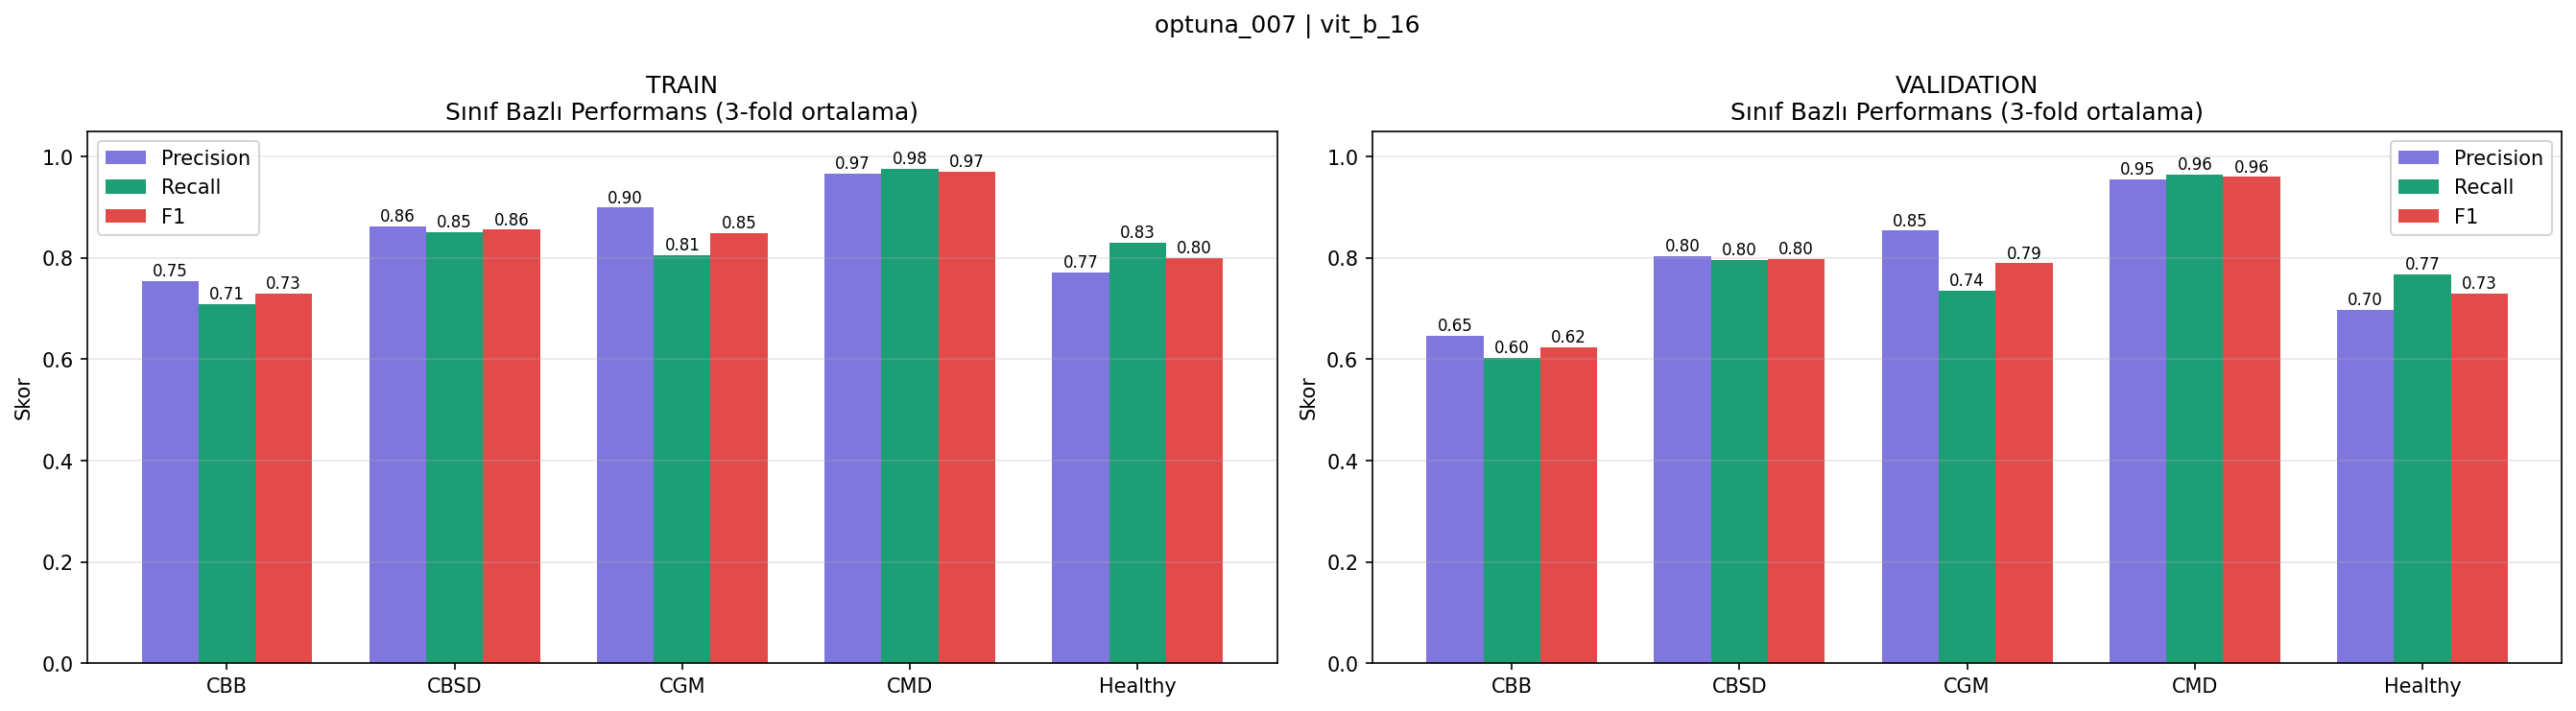
\includegraphics[width=\linewidth]{fig/fig_perclass_best_dl.png}
\caption{Per-class precision, recall, and F1 of the selected best deep-learning trial (mean across 3 folds). The model handles CMD almost perfectly ($F_1 \approx 0.96$) but is weakest on CBB ($F_1 \approx 0.63$), the rarest class.}
\label{fig:perclass}
\end{figure}

\begin{figure}[t]
\centering
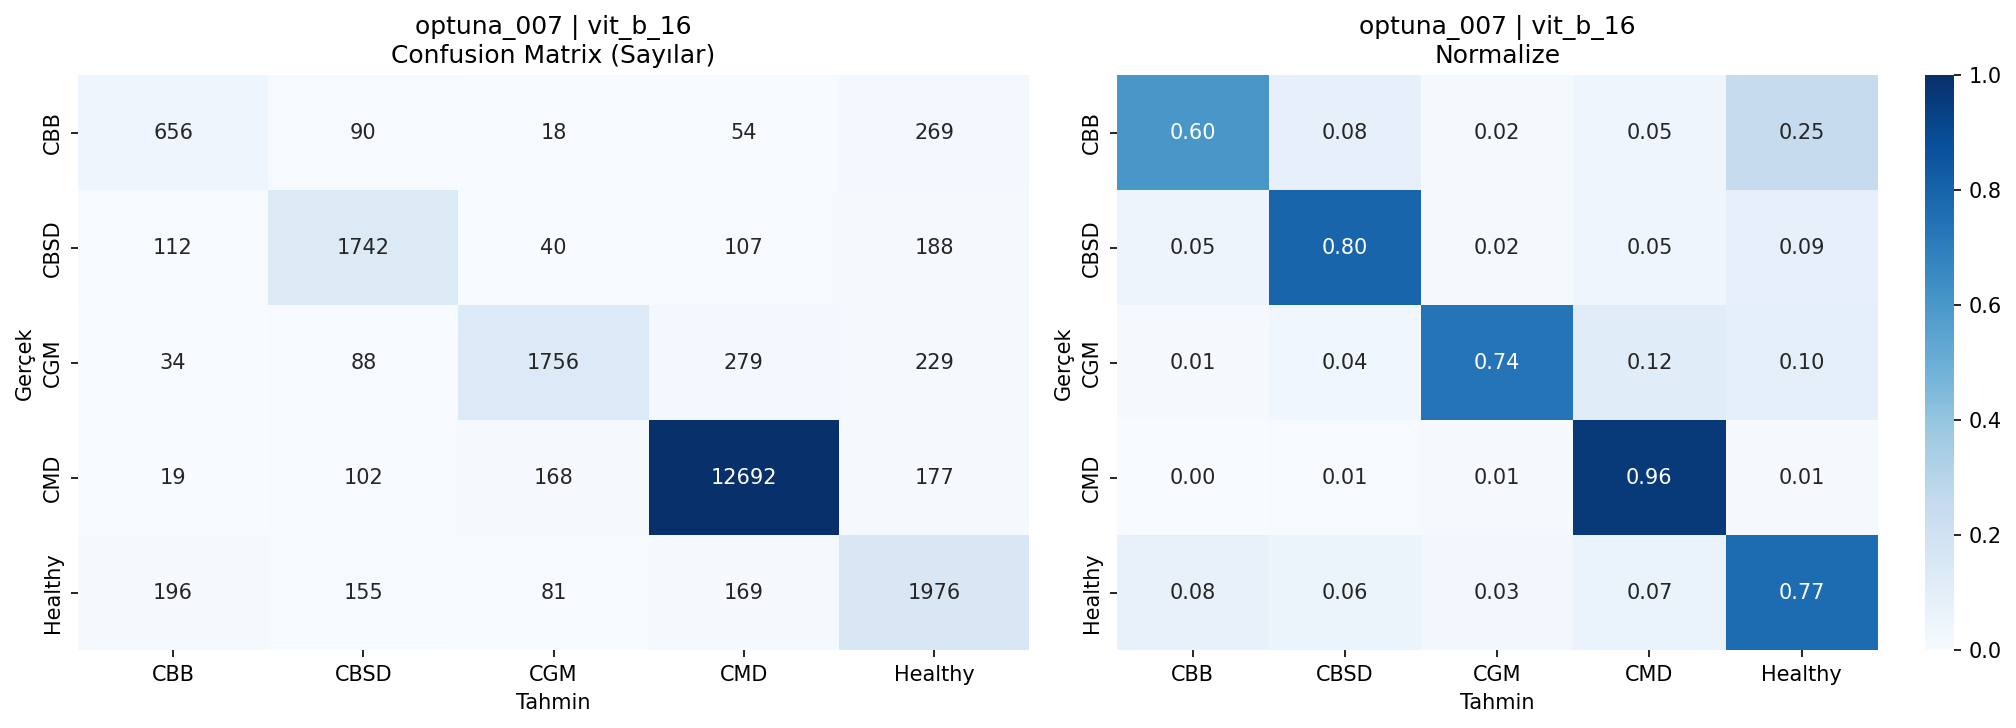
\includegraphics[width=\linewidth]{fig/fig_cm_best_dl.png}
\caption{Confusion matrix of the selected best deep-learning trial (out-of-fold predictions aggregated across 3 folds). Most off-diagonal mass for CBB and Healthy is absorbed into CMD, the dominant class.}
\label{fig:cm_best}
\end{figure}

\begin{figure}[t]
\centering
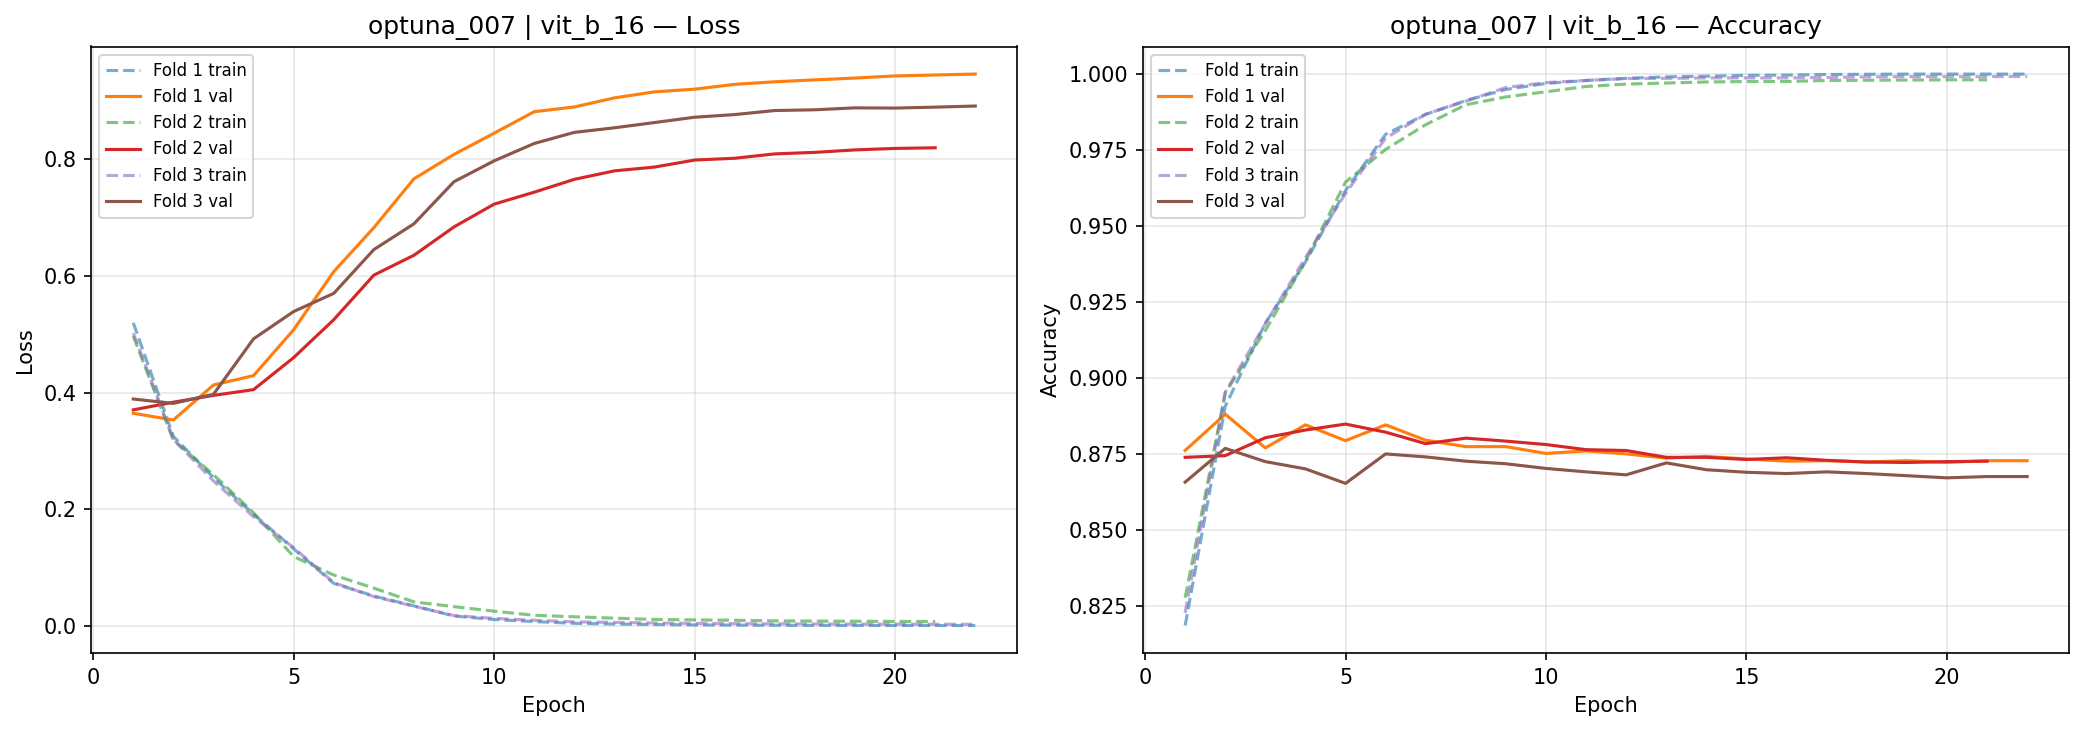
\includegraphics[width=\linewidth]{fig/fig_curves_best_dl.png}
\caption{Training and validation loss/accuracy curves for the selected best trial across the three folds. Convergence is extremely fast (best epoch within $[1,2]$ on every fold), after which validation loss diverges from training loss; the early-stopping criterion restores the best validation checkpoint before final evaluation.}
\label{fig:curves}
\end{figure}

A notable observation is that the best validation epoch falls in the range $[1, 2]$ on all three folds, despite the $200$-epoch budget and patience $20$. This indicates that fine-tuning a fully ImageNet-pretrained ViT on CLDC saturates extremely quickly: after roughly two epochs of full-network adaptation, additional epochs only increase the train--validation gap. The current best deep-learning trial reaches accuracy $\approx 0.88$, which is meaningfully below state-of-the-art ensembled solutions on this benchmark (top-1\% Kaggle solutions reach $\approx 0.91$); closing this gap is one of the explicit motivations for the upcoming augmentation ablation.

\subsection{Per-Class Behavior and Hardest Class}
Across every leading trial in Tables~\ref{tab:results_cnn} and~\ref{tab:results_vit}, the per-class metrics follow the same pattern. CMD is essentially solved ($F_1 \approx 0.96$), CBSD and CGM reach the high $0.75$--$0.80$ range, Healthy lies near $0.72$, and CBB is consistently the hardest class with $F_1 \approx 0.63$ at best. Two factors are responsible. First, CBB has only $1{,}087$ training images (about one-twelfth of CMD), so even balanced reweighting cannot fully compensate for the limited intra-class diversity. Second, the visual symptoms of CBB (angular leaf spots) overlap with both Healthy and CGM under varying illumination, which puts a hard ceiling on the achievable per-class F1 without targeted augmentation. These observations directly motivate the augmentation ablation summarized in Section~\ref{ssec:ablation}, which is currently in progress.

% =====================================================================
% Bibliography
% =====================================================================
\bibliographystyle{IEEEtran}
\bibliography{references}

\end{document}
